\documentclass[11pt,twoside,a4paper,final]{book}
\usepackage[left=1.6in,right=1.6in,top=1.6in,bottom=1.6in]{geometry}
\usepackage{graphicx}
\usepackage{hyphenat}
\usepackage{todonotes}

\title{zkSwap - Scaling Decentralized Exchanges through Transaction Aggregation}
\author{Paul Etscheit}
\date{March 2021}

\begin{document}

\begin{titlepage}
\maketitle
\end{titlepage}

\section{Introduction}
When being launched in 2015, Ethereum \cite{wood2014ethereum} set out to change the way we compute. A trustless, permissionless, and decentralized world computer was envisioned, set to open a new class of applications. The importance of running verifiable, Turing-complete code in a permissionless and trustless manner cannot be overstated and enables products and services not thought to be possible. However, the technical limitations have also become apparent quickly. Computations are expensive, theoretical transactions per second are low, and the overall throughput has been stagnant. While Eth2 gives a path towards scaling the network, it is expected to take years to complete. 

The first major use case for Ethereum was tokenization. With the development of the ERC-20 standard, launching a token on the Ethereum blockchain was trivial. As tokens run as smart-contracts on the Ethereum blockchain, they are secured by its proof of work consensus, which, given Ethereums PoW hash rate, makes consensus attacks infeasible. Running on Ethereum blockchain is a significant benefit when looking to tokenize things, as network security can be assumed. While tokenizations are a step in the right direction, they do not come close to the initial vision. While the standardization enables simple integrations into exchanges and wallets, most tokens are isolated in their functionality and ecosystem and lack productive usage.
\todo{token all isolated, not working together... Not a lot of gas needed blabla}

With all of these developments over the past couple of years, it seems we have now entered a new phase of smart-contract use-cases, namely Decentralized Finance (DeFi). While DeFi has many different products and functionalities, at its core aims to utilize tokenized assets in some productive form. 


Lending and collateralized borrowing is possible with Aave \cite{kulechov_2020}, assets can be deposited into liquidity pools\cite{adams2020uniswap} to generate yields, flash-loans \cite{kulechov_2020}\cite{adams2020uniswap} enabled uncollateralized borrowing as long as the loan is repaid in the same transaction and assets can be traded in a non-custodial way with Uniswap \cite{adams2020uniswap} \todo{Mention other swap protocols?}. It can be questioned how useful or necessary these protocols really are, but the core idea behind them is impressive. Rebuilding traditional financial products, running as non-custodial and permission-less smart-contracts, all based on the same standardizations, has the potential to reshape the way finance works. With these developments not looking to slow down, they are quickly overwhelming the Ethereum blockchain, pushing transaction costs \cite{gasprice} higher and higher. 

One of these new DeFi applications is Uniswap \cite{adams2020uniswap}. Uniswap is a crypto-asset exchange running as a collection of smart-contracts on the Ethereum blockchain, enabling non-custodial, trust-less, and permission-less trading of ERC-20 assets. Since its running on the Ethereum Blockchain, reducing the computational complexity of trade execution is essential for making it a viable product. In typical crypto-asset exchanges, trading is built around a central order book. Users can add buy or sell orders for a given trading pair, and a matching engine checks if these orders can be matched, executing the trade once they do. While running this on modern server infrastructure is feasible, running it on the blockchain is not. The demand for memory and processing power is too large, so a different approach must be taken. Uniswap solves this by applying the automated market maker (AMM) model, which will be explained in detail in sec. XX. By applying this model, Uniswap reduces the computational complexity to make this a viable business model. At least it was, when Uniswap launched. 

\begin{figure}[h]
    \centerline{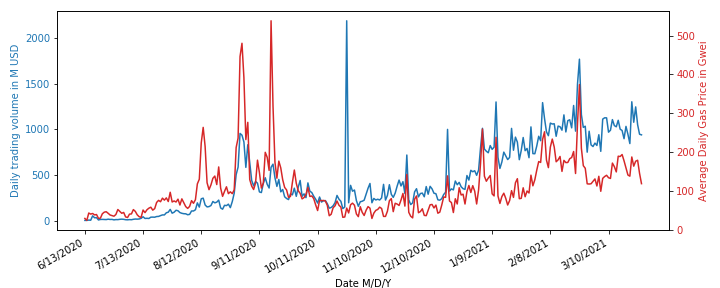
\includegraphics[totalheight=5.6cm]{diagrams/gas_volume.png}}
    \caption{Combined daily Uniswap trading volume in million USD and average daily Ethereum gas price}
    \label{fig:gas_vol}
\end{figure}

The recent rise of Ethereums gas price \cite{gasprice} can also be attributed to the growing popularity of Uniswap. Currently, it is one of the most used smart-contract on the Ethereum blockchain, making up on average around 15\% of gas \cite{eth_gas_guzzlers} usage of a block at the time of writing. To date, it accrued over \$280 million in transaction fees \cite{uniswap_tx_fees} and has settled over \$100 billion in trading volume \cite{cummulative_vol}. With the gas price having reached 500 gwei on a couple of occasions, a single Uniswap trade can cost upwards of \$130. While it would be assumed that high gas prices cause a reduction in trading volume, the opposite is the case. As shown in F.\ref{fig:gas_vol} there seems to be a strong correlation between daily trading volume on Uniswap and the average daily Ethereum gas price, so reducing gas consumption by Uniswap transactions should result in a reduced gas price for the entire network.

With longer-term scaling solutions in development but still years away, a shorter-term solution is needed. A couple of short-term scaling approaches have been proposed. While these do differ, they all aim to move transactional data to a layer-2\footnote{A layer-2 system is a data storage that does not reside on the blockchain but has its state committed to it in some way} system, while ensuring correctness of that data in some way. One of the approaches is called zk-rollup, the focus of this work. Moving data to a layer-2 system can increase the number of transactions that fit into a block while also reducing transaction costs for the user, with is beneficial for Uniswap users and all other participants of the Ethereum network. 

Current zk-rollup enabled applications running on the Ethereum mainnet, one of them being ZK Sync, are focused on reducing cost of Ether and ERC-20 transfers\todo{not a great sentence}. Users deposit funds into its smart-contract, which results in the user's deposit being represented as balance in layer-2. When a user makes a transfer to another user, the involved balances get updated in layer-2, while the correctness of these updates is ensured via zkSNARK. It is important to note, that ZK Sync acts as a closed system, transfers only change balances in layer-2, while deposited funds in the smart-contract do not move. While this approach has significantly reduced costs of transfers, it only marks the first generation of potential(?) zk-rollup enabled apps.

Aggregating Uniswap trades is an interesting application to explore the potential of zk-rollup technology. It combines the layer-2 storing and updating of balances already done by ZK Sync while opening the system to interact with other smart-contracts. When aggregating trades, we need to interact with the Uniswap contracts to execute the aggregated trade, then update the layer-2 balances according to the trade and verify everything via zkSNARK. It is the next step in exploring the potential of zk-rollups as a generalizable scaling solution, applicable to any kind of smart-contract. 


\section{Background}
% good idea for introducing gas as power/efficiency metric

% When discussing scaling, gas is a good metric to look at. Every block in Ethereums blockchain has a gas limit that can't be oversteped, \todo{check this, miners should be able to seal blocks still i think} so its a good indicator of proccessing power of the network. At the same time, transactions with smart-contracts use an amount of gas for there execution. The amount of gas needed is defined by the opcodes used for that transaction, which have a fixed price. In that sense, a smart-contracts efficiency can be defined by the amount of gas needed for a transaction. 

% As with all computer systems, scaling can be achived by increasing processing power. Increasing the processing power of a distributed system however, is a complex process. Given that the system is optimized, the only real approach to increasing processing power is sharding. Conceptually, sharding can be seen as upgrading to a multi-core CPU. We seperate the network into individual shards, not requiring every node to proccess every transaction, thereby increasing the processing power of the entire network. Transitioning to a sharded network, namely Eth2, is a highly complex process expected to take years to complete. While this is an inevitable step, aimed at increasing the networks processing power, it wont help in scaling the network for the next couple of years. Shorter term solutions are needed. 

% Another approach for scaling is increasing a smart-contracts efficiency. As in traditional software applications, reducing the computational cost per operation will in general increase our throughput. In smart-contracts this can be achived by reducing the amount of gas needed for a executing a transaction. As every block has a maximum amount of gas that can be proccessed, reducing it will result in an increased amount of transactions to be proccessed in that block. In smart-contracts data-storage is very expensive. To reduce cost

\subsection{zk-rollup}
Zk-rollup \cite{vbuterin_2018} is a layer-2 scaling approach first introduced as a technique to mass validate transfers of assets in 2018. The system described consists of two types of users, transactors and an relayer. To make transfers, a transactors first need to deposit funds into the systems contract. 


When depositing, the user need to provide a valid merkle path to its current balance in the system, which might be null, or include previously deposited funds or received transfers. If the path is valid, the balance is updated and emitted via the event log. The balance has now been moved to layer-2. A transactor can withdraw funds from the smart contract, by providing a valid merkle path and the withdraw amount. As the balance object, previously emitted as an event includes the users address, the transactions sender address is used, when checking the merkle proof. This ensures the transactor controlles the private key of that address.


When making a transfer, it is sent as an http request to the relayer. The 


\section{Design}
The implementation of this system consist of a number of entites, that are required to aggregate and execute trades in a trust-less and non-custodial manner, while not having any data availability issues\todo{Need to find a better word for data availablilty issues}. As a first step, the smart-contracts used for depositing and withdrawing funds into the system will be explained. The second step will introduce the off-chain entity, that is tasked with aggregating, executing and verifying the trades.

\subsection{System Overview}
The system consists of two main entites that are required for it to function. The first entity to look at, is the on-chain entity, we call zkSwap. zkSwap is a smart-contract deployed on the Ethereum blockchain and has three main jobs, processing deposits and withdraws, aswell as verifying batched trades. As our goal is to not rely on external data-availability, while remaining trust-less and non-custodial, the zkSwap contract is the only entity that can change the state stored in layer-2, by emitting state updates via the event log. Since the event log can be extracted from the blockchain by clients, it is always accessible, while being signficantly cheaper then storing data as a variable in a smart-contract.

The second entity to look at is the aggregator. The aggregator consists numerous systems, both off-chain and on-chain, and is mainly tasked with receiving trade orders, batching and executing them, and then verifying them with the zkSwap contract. The aggregator stores a merkle-tree of users balances and keeps it in sync by listening for event emitted by the zkSwap contract. 

% \subsection{Entity Interactions}
% To understand how the system works, the first thing to understand is how these two entites interact. As mentioned before, the zkSwap contract is the only state-changing entity in this system. It is the single source of truth

\subsection{Zk-Rollup Explained}


\subsection{zkSwap Contract}
Since we're looking to aggregate Uniswap trades, the obvious functionality required is for users deposit and withdraw funds, which will then in turn be used for trading. Users can deposit or withdraw funds by sending the corresponding transactions to the zkSwap contract, which will then


As mentioned before, the zkSwap contract is the only state-changing entity in this system. All state-changing operations are checked and then committed by this contract. This might be counter intuitive at first, as the goal is to move as much data as possible off-chain. It is important to remember though, that one main goal is not to rely on any external data availibility. This can only be achived by storing state on-chain, as compressed as possible. 

At the center of storing state is our system, is the root of the balance merkle tree, stored in the zkSwap contract. 


Since we're looking to aggregate Uniswap trades, the obvious functionality required is for users deposit and withdraw funds, which will then in turn be used for trading. As we're looking to move as much data as possible to layer-2. 




As the goal is also for this to remain trust-less and non-custodial, while not relying on any data availability



, while moving the balance to layer-2 the smart-contract need to be able to verify these transactions, while emitting enough data,

As the goal for this system is to be trust-less and non-custodial the first thing to look at, 



When looking to move data off-chain, a smart-contract is needed. De

Since the main goal is to move data off-chain, the first thing to look at is now 


As a first step the smart-contracts used for depositing and withdrawing funds, will be introduced. In the second 




Goal of this system, is to introduce a trust-less and non-custodial 


\bibliographystyle{splncs04}
\bibliography{mybibliography}
\end{document}
